%%% Sample chapter with examples of tables, figures, and code

\chapter{Tables, Figures, Code Listings}

Using tables and graphs/figures in academic text has some rules in common and some that are specific. We do not place tables and graphs/figures directly in the text, but on a separate page or in a reserved spot at the top or bottom of a normal page. \LaTeX\ takes care of the placement of floating graphs and tables automatically.

Graphs/figures and tables are numbered and carry a caption. The caption should describe the content of the graph or table in enough detail that the reader understands it without carefully studying the thesis text.

Every table and graph/figure must be referenced by number in the text (the dynamic cross-referencing mechanism built into \LaTeX\ is strongly recommended). At the relevant point in the text, summarize the most important conclusions that can be drawn from the table or graph. The text should be readable and understandable even without looking at the tables and graphs, and the tables and graphs should be understandable even without a detailed reading of the text.

Where possible, refer to tables and graphs indirectly as part of the normal flow of the text; instead of \emph{\enquote{Table~\ref{tab03:Estimates} shows that
    men are on average $9.9\,\rm kg$ heavier than women}} write
\emph{\enquote{Men are $9.9\,\rm kg$ heavier than women on average (see
    tab.~\ref{tab03:Estimates})}}.

\section{Tables}

\begin{table}[htbp!]

\centering
%%% This table uses the following packages:
%%%   - booktabs (\toprule, \midrule, \bottomrule)
%%%   - dcolumn (column type D: numbers centred and aligned on the
%%%     decimal point)

\caption{Maximum-likelihood estimates in model M.}\label{tab03:Estimates}
\begin{tabular}{lD{.}{.}{3.2}D{.}{.}{1.2}D{.}{.}{2.3}}
\toprule
               &                & \multicolumn{1}{c}{\textbf{Std.}}   &  \\
\textbf{Effect} & \multicolumn{1}{c}{\textbf{Estimate}} & \multicolumn{1}{c}{\textbf{error}$^a$} & \multicolumn{1}{c}{\textbf{P-value}} \\
\midrule
Intercept     & -10.01 & 1.01 & \multicolumn{1}{c}{---} \\
Sex (male)    & 9.89   & 5.98 & 0.098 \\
Height (cm)   & 0.78   & 0.12 & <0.001 \\
\bottomrule
\multicolumn{4}{l}{\footnotesize \textit{Note:}$^a$ Standard error of the estimate obtained by the Monte Carlo method.}
\end{tabular}
\end{table}

The following rules are recommended for \textbf{tables}:

\begin{itemize} %% or compactitem from the paralist package
\item Avoid vertical rules. Use heavier horizontal rules to separate
  the table from the surrounding text, including the caption, and
  lighter horizontal rules to separate the column headers from the
  body of the table and the individual parts of the table from each
  other. In \LaTeX\ this style of table is implemented by the
  \texttt{booktabs} package. If some columns need to be more clearly
  separated from others, insert a larger gap between them.
\item Do not change the type, format, or meaning of the content of
  cells within the same column (it is not good to put an average in
  one row of a column and a percentage in another).
\item Do not repeat the same cell content many times in a row. If we
  have a column \textit{Variance} that contains the value $0.5$ in
  the first ten rows and the value $1.5$ in the next ten rows, it is
  better to remove that column and solve it another way. For example,
  we can split the table into two, or insert descriptive rows that
  state some variable value that recurs across the following section
  of the table (e.g. \emph{\enquote{Variance${}=0.5$}} and below
  \emph{\enquote{Variance${}=1.5$}}).
\item Align numbers in a table on the decimal point.
\item A table sometimes needs to use abbreviations that do not occur
  elsewhere. These abbreviations can be explained in the caption or
  in notes below the table. Notes below the table can also be used to
  explain the meaning of certain columns or values in more detail.
\end{itemize}


\section{Figures}

\begin{figure}[htbp!]\centering
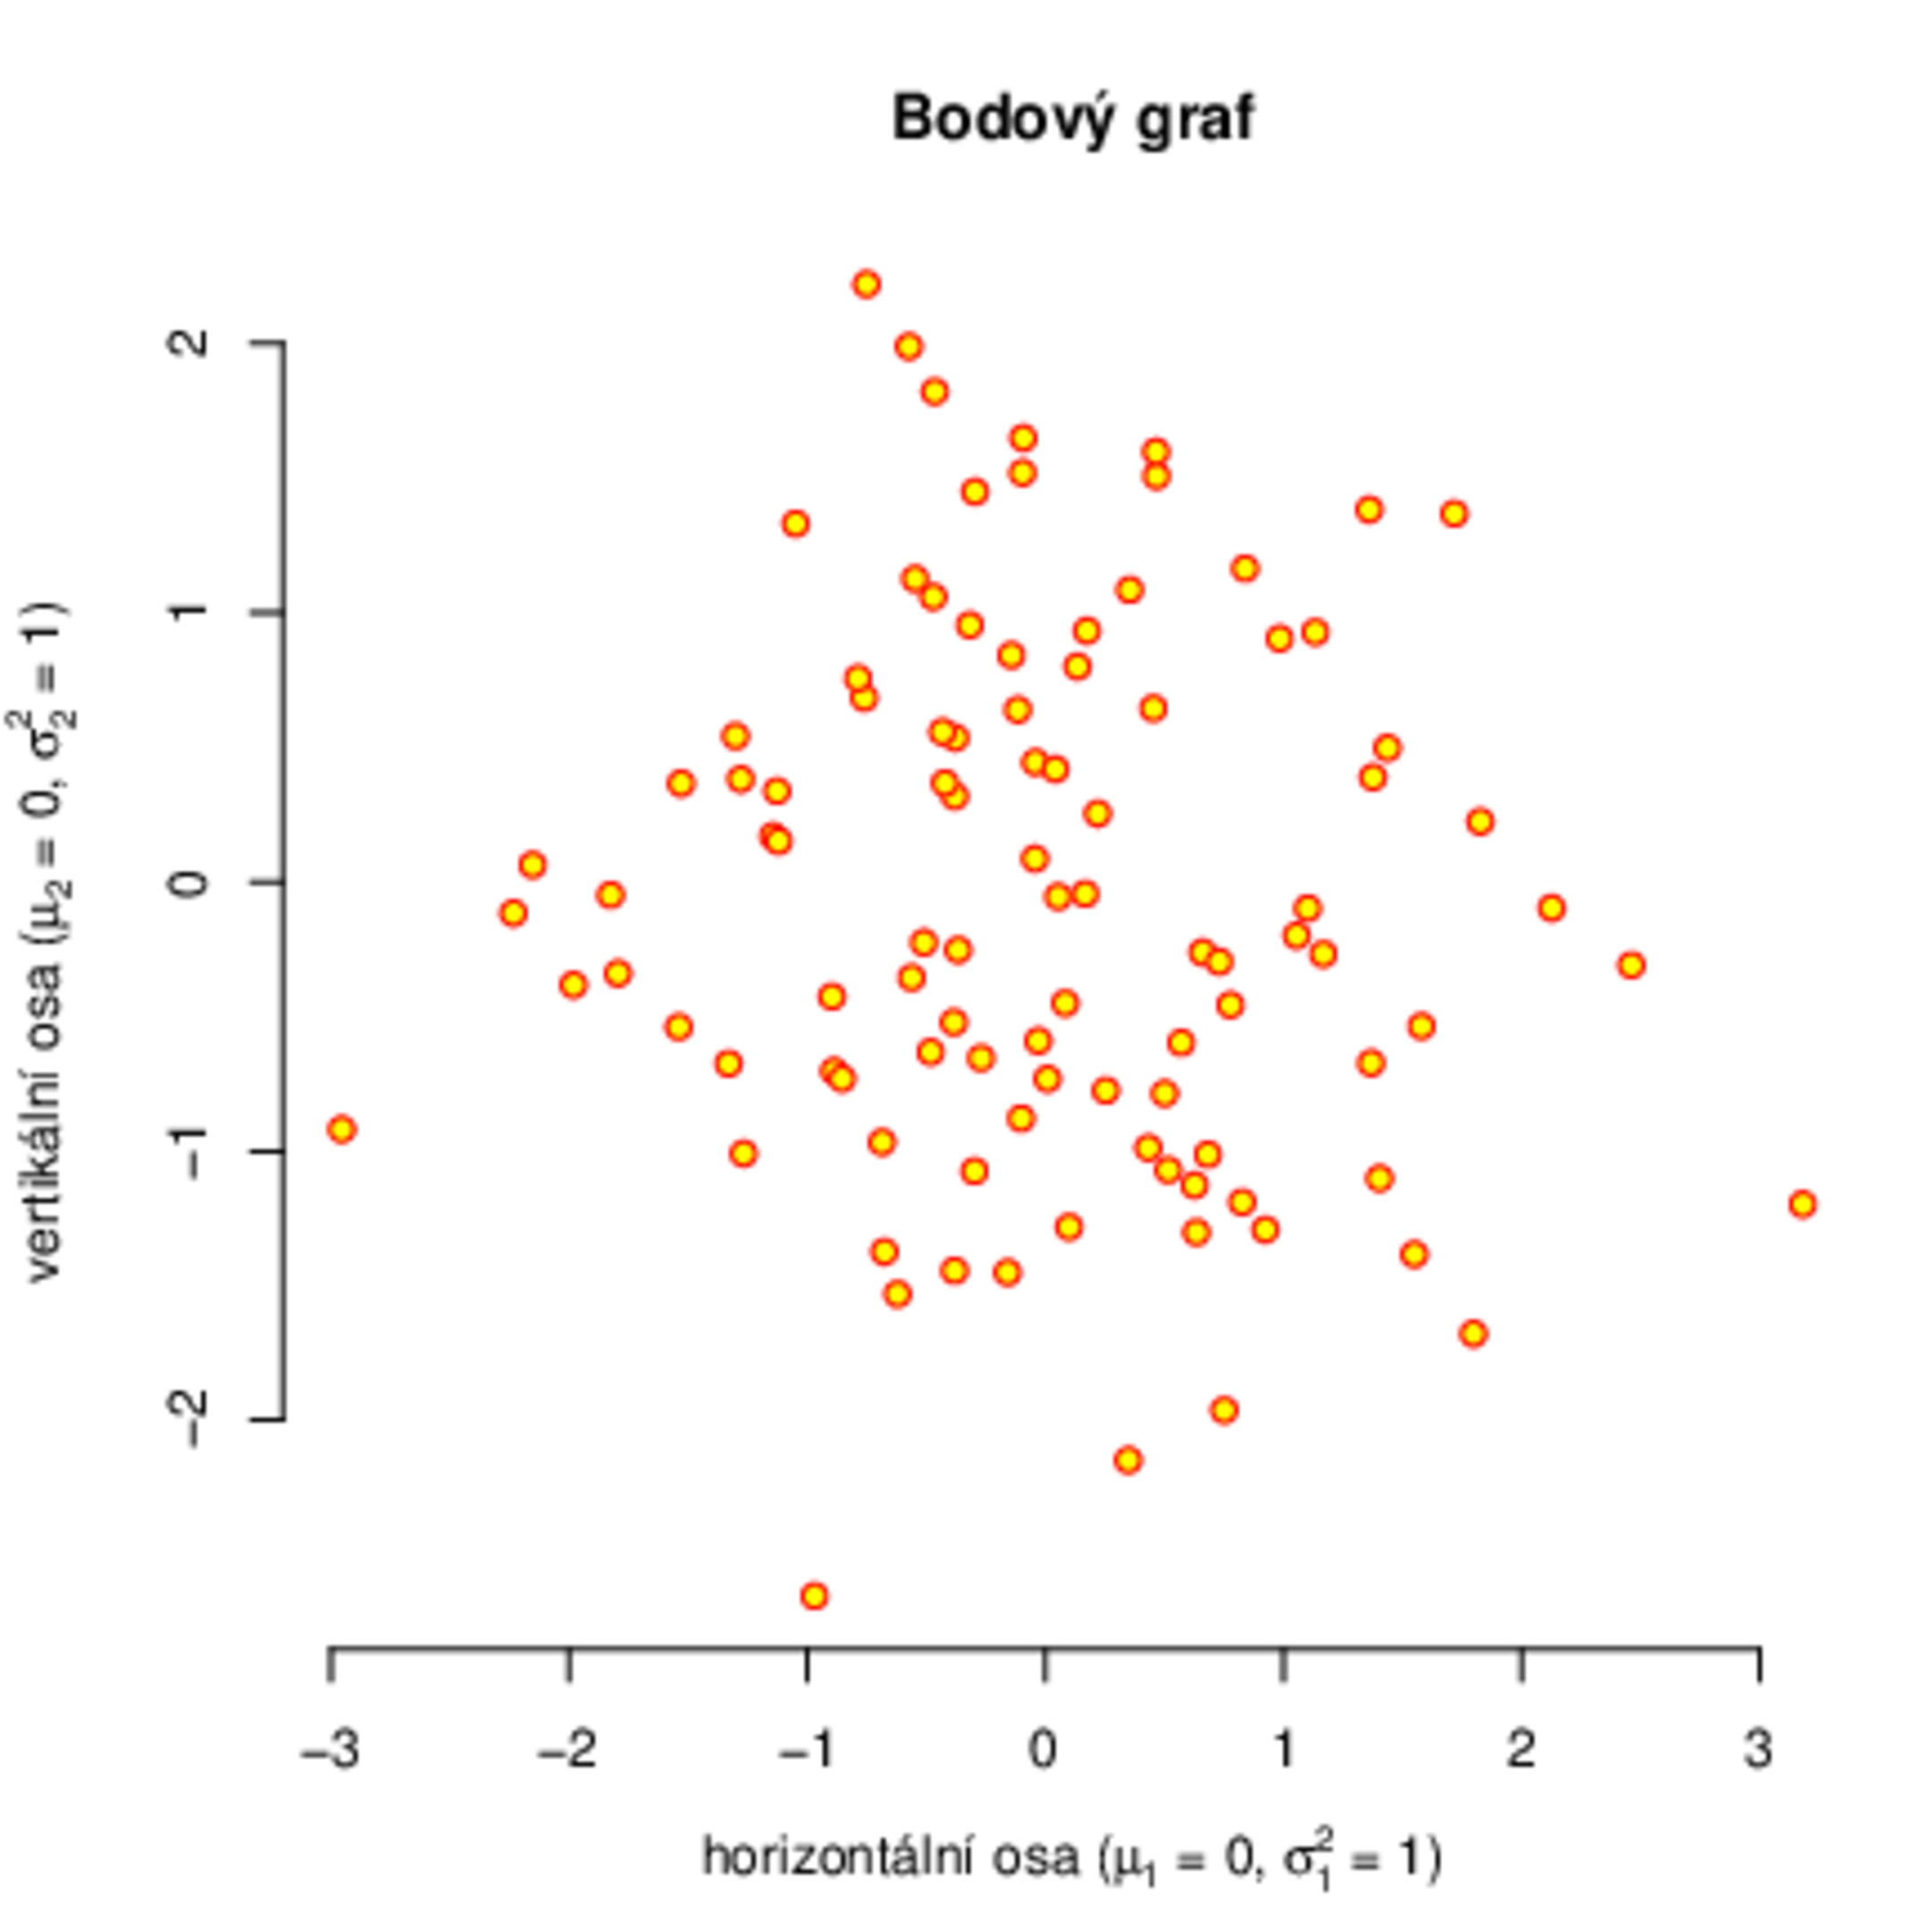
\includegraphics[width=.66\textwidth]{figures/example-fig01}
% There is no need to state the extension explicitly, pdflatex looks for a pdf automatically.
% There is also no need to state the dimensions.
\caption{A random sample from the distribution $\mathcal{N}_2(\boldsymbol{0},\,I)$.}
\label{fig03:Sample}
\end{figure}

A few pieces of advice regarding figures and graphs.

\begin{itemize}
\item A graph should be created at the size at which it will be used
  in the thesis. Shrinking a graph that is too large leads to poor
  label legibility.
\item The axes of a graph must be properly labelled in the same
  language the thesis is written in (missing diacritics can be
  tolerated). If plotting weight against height, don't leave the
  labels as \texttt{ht} and \texttt{wt}; instead label the axes
  \emph{Height [cm]} and \emph{Weight [kg]}. If plotting a function
  $h(x)$, label the axes $x$ and $h(x)$. Every axis must have a
  clearly defined scale.
\item If you need to mark a large number of points on a
  two-dimensional graph, make sure they do not merge into a solid
  black mass. If there are many points, reduce the size of the symbol
  used to plot them, or select only a small subset of the points to
  include in the graph. Graphs containing thousands of points cause
  problems especially in electronic documents, because they
  significantly increase file size.
\item If the thesis will be printed in black and white, avoid using
  colour. Distinguish lines by their style (solid, dotted,
  dash-dotted, \ldots), and areas by sufficiently different
  intensities of grey or by hatching. Explain the meaning of the
  individual line and area styles either in a text caption for the
  graph or in a graphical legend that is part of the figure itself.
\item Avoid low-resolution bitmap images, and JPEGs in particular
  (jagged edges and compression artefacts don't look good on paper).
  It is better to create images as vector graphics and insert them
  into the text as PDF (watch out for the PDF/A issue described in
  chapter~\ref{chap:pdfa}).
\end{itemize}


\section{Source Code}
Algorithms, program listings, and descriptions of program interaction are best set apart from the rest of the text. \texttt{upsgthesis.cls} defines a \texttt{code} environment on top of the \texttt{listings} package for this, with syntax highlighting for whichever language you name as its optional argument, e.g.\ \verb|\begin{code}[Python]|. Leave the argument out for plain, unhighlighted text -- useful for console transcripts such as the following. Longer or supplementary source code belongs in an appendix instead (see appendix~\ref{app:code}, which also shows a highlighted Python example).

\begin{code}
> mean(x)
[1] 158.90
> object$mean
[1] 158.90
\end{code}

\texttt{listings} is very richly configurable well beyond what this template sets up by default -- see its documentation, or:
\begin{itemize}
\item \url{https://en.wikibooks.org/wiki/LaTeX/Source_Code_Listings}
\item \url{https://www.overleaf.com/learn/latex/Code_listing#Using_listings_to_highlight_code}
\end{itemize}


\section{Typesetting Mathematics}
Variables are set in italics (\TeX{} does this automatically in math mode, but don't forget it in the surrounding text either, and remember to switch on math mode). Function names are set upright. For example:
$\textrm{var} (X) = \textsf{E~} X^2 - \bigl(\textsf{E~} X \bigr)^2$.

Fractions within a paragraph (such as $\frac{5}{7}$ or $\frac{x+y}{2}$) can be too cramped, so it is better to typeset simple fractions with a slash: $5/7$, $(x+y)/2$.

\LaTeX's options for typesetting mathematics are rich, but it is possible that in some specific situations they won't be sufficient. In that case, the American Mathematical Society (AMS) packages are recommended. The packages \texttt{amsmath}, \texttt{amsfonts}, and \texttt{amsthm} are loaded by default in \texttt{upsgthesis.cls}. To explore their capabilities further, see:
\begin{itemize}
\item Math Extension with AMS\LaTeX\ -- \url{http://ptgmedia.pearsoncmg.com/images/0321173856/samplechapter/kopkach15.pdf}
\item \url{https://www.overleaf.com/learn/latex/Aligning_equations_with_amsmath}
\item Math Mode -- \url{http://tex.loria.fr/general/Voss-Mathmode.pdf}
\item More Math into LaTeX -- \url{http://tug.ctan.org/info/Math_into_LaTeX-4/Short_Course.pdf}
\end{itemize}
